\documentclass[tikz,border=8pt]{standalone}
\usepackage{amsmath}
\usetikzlibrary{arrows.meta}
\definecolor{ink}{HTML}{21352F}
\definecolor{teal}{HTML}{087F7B}
\definecolor{blue}{HTML}{4B77A8}
\definecolor{gold}{HTML}{C58B2A}
\begin{document}
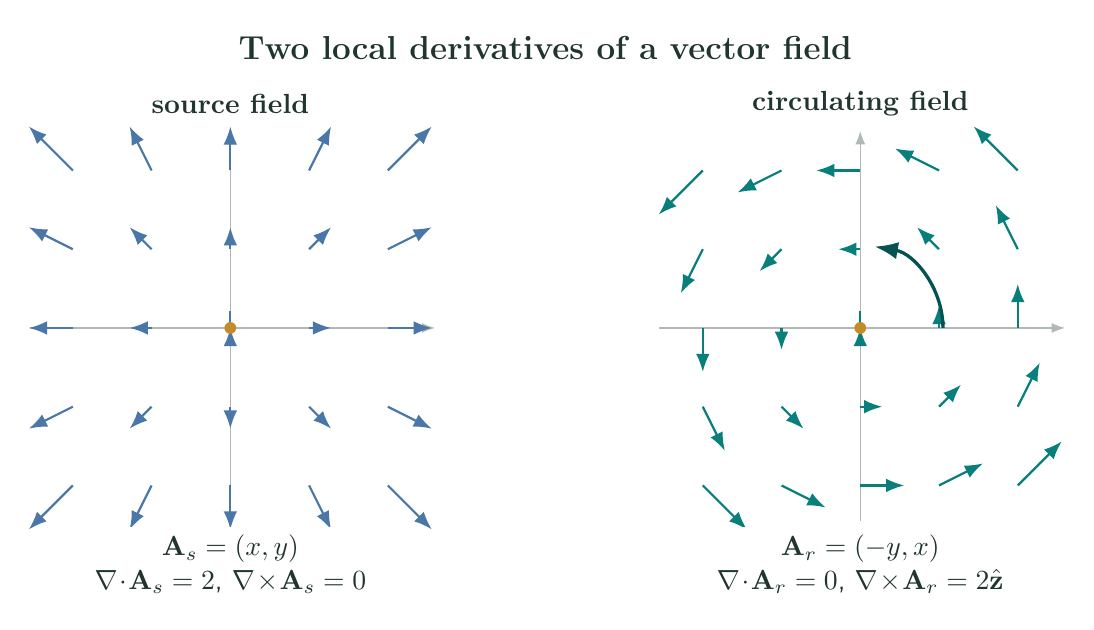
\begin{tikzpicture}[font=\sffamily,text=ink,>=Latex]
  \node[font=\bfseries\large] at (0,3.55)
    {Two local derivatives of a vector field};

  \begin{scope}[xshift=-4.0cm]
    \node[font=\bfseries] at (0,2.85) {source field};
    \draw[->,ink!35] (-2.55,0)--(2.6,0);
    \draw[->,ink!35] (0,-2.45)--(0,2.5);
    \foreach \x in {-2,-1,0,1,2}{
      \foreach \y in {-2,-1,0,1,2}{
        \pgfmathsetmacro{\dx}{0.28*\x}
        \pgfmathsetmacro{\dy}{0.28*\y}
        \draw[blue,thick,->] (\x,\y)--++(\dx,\dy);
      }
    }
    \fill[gold] (0,0) circle (.075);
    \node[align=center,fill=white,inner sep=3pt] at (0,-3.0)
      {$\mathbf A_s=(x,y)$\\
       $\nabla\!\cdot\!\mathbf A_s=2$,
       $\nabla\!\times\!\mathbf A_s=0$};
  \end{scope}

  \begin{scope}[xshift=4.0cm]
    \node[font=\bfseries] at (0,2.85) {circulating field};
    \draw[->,ink!35] (-2.55,0)--(2.6,0);
    \draw[->,ink!35] (0,-2.45)--(0,2.5);
    \foreach \x in {-2,-1,0,1,2}{
      \foreach \y in {-2,-1,0,1,2}{
        \pgfmathsetmacro{\dx}{-0.28*\y}
        \pgfmathsetmacro{\dy}{0.28*\x}
        \draw[teal,thick,->] (\x,\y)--++(\dx,\dy);
      }
    }
    \fill[gold] (0,0) circle (.075);
    \draw[teal!65!black,very thick,->] (1.05,0)
      arc[start angle=0,end angle=80,radius=1.05];
    \node[align=center,fill=white,inner sep=3pt] at (0,-3.0)
      {$\mathbf A_r=(-y,x)$\\
       $\nabla\!\cdot\!\mathbf A_r=0$,
       $\nabla\!\times\!\mathbf A_r=2\hat{\mathbf z}$};
  \end{scope}
\end{tikzpicture}
\end{document}
